\documentclass{article}
\usepackage{booktabs}
\usepackage{array}
\usepackage[margin=0.6in, landscape]{geometry}
\usepackage[table]{xcolor}
\usepackage{colortbl}
\usepackage{tikz}
\usepackage{enumitem}
\usepackage{amssymb}
\usepackage{makecell}

\definecolor{BrightGreen}{RGB}{0,204,0}
\definecolor{Chocolate}{RGB}{123,63,0}

\begin{document}

%───────────────────────────────────────────────
%  PAGE 1 — Main Payment Summary
%───────────────────────────────────────────────

\begin{center}
\LARGE\textbf{Mess Meal Management System}\\[4pt]
\Large September 2026 \quad Payment Summary
\end{center}

\vspace{0.4cm}

\begin{table}[h]
\centering
\normalsize
\renewcommand{\arraystretch}{1.8}
\setlength{\tabcolsep}{7pt}
\begin{tabular}{l r r r r r r r r r r r r r l}
\toprule
\rowcolor{blue!20}
\textbf{Name} &
\makecell{\textbf{Bazar}\\(BDT)} &
\makecell{\textbf{Meal}\\Cost} &
\makecell{\textbf{Have to}\\Pay} &
\makecell{\textbf{Khala}\\Bill} &
\makecell{\textbf{House}\\Rent} &
\textbf{WiFi} &
\textbf{Gas} &
\makecell{\textbf{Init.}\\Cost} &
\makecell{\textbf{Have to Pay}\\(Init. Cost)} &
\makecell{\textbf{Prev.}\\Due} &
\makecell{\textbf{Sub-}\\total} &
\makecell{\textbf{Extra}\\Pay} &
\makecell{\textbf{Final}\\Pay} &
\textbf{Status} \\
\midrule
\rowcolor{gray!10}
Ayman & 2,066 & 1,599 & $-467$ & 1,125 & 4,375 & 162.50 & 115.00 & 63.75 & $-56.25$ & 0 & 5,254.00 & 75.00 & \cellcolor{green!30}\textbf{5,330.00} & \textcolor{red}{Unpaid} \\
\rowcolor{white}
Saad  & 2,028 & 2,251 & $+223$ & 1,125 & 3,750 & 162.50 & 115.00 & 63.75 & $+63.75$ & 0 & 5,439.00 & 75.00 & \cellcolor{green!30}\textbf{5,515.00} & \textcolor{red}{Unpaid} \\
\rowcolor{gray!10}
Alif  & 2,234 & 2,349 & $+115$ & 1,125 & 4,375 & 162.50 & 115.00 & 63.75 & $-71.25$ & 0 & 5,821.00 & 75.00 & \cellcolor{green!30}\textbf{5,900.00} & \textcolor{red}{Unpaid} \\
\rowcolor{white}
Asif  & 0 & 131 & $+131$ & 1,125 & 3,000 & 162.50 & 115.00 & 63.75 & $+63.75$ & 0 & 4,597.00 & 75.00 & \cellcolor{green!30}\textbf{4,675.00} & \textcolor{red}{Unpaid} \\
\midrule
\rowcolor{green!30}
\textbf{Total} & \textbf{6,328} & \textbf{6,330} & \textbf{2} & \textbf{4,500} & \textbf{15,500} & \textbf{650.00} & \textbf{460.00} & \textbf{255} & \textbf{0} & \textbf{0} & \textbf{21,111.00} & \textbf{300.00} & \textbf{21,420.00} & \\
\bottomrule
\end{tabular}
\end{table}

\vspace{0.4cm}

%───────────────────────────────────────────────
%  Bottom section: 3 columns
%───────────────────────────────────────────────

\begin{minipage}{0.24\textwidth}
\centering
{\large\textbf{\underline{Final Pay Summary}}}\\[6pt]
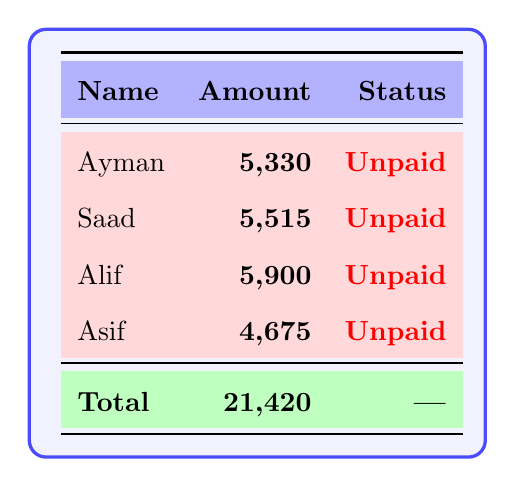
\begin{tikzpicture}
\node[draw=blue!70, very thick, rounded corners=6pt, fill=blue!5, inner sep=8pt] {
\renewcommand{\arraystretch}{1.7}
\begin{tabular}{lrr}
\toprule
\rowcolor{blue!30}
\textbf{Name} & \textbf{Amount} & \textbf{Status} \\
\midrule
\rowcolor{red!15}
Ayman & \textbf{5,330} & \textcolor{red}{\textbf{Unpaid}} \\
\rowcolor{red!15}
Saad  & \textbf{5,515} & \textcolor{red}{\textbf{Unpaid}} \\
\rowcolor{red!15}
Alif  & \textbf{5,900} & \textcolor{red}{\textbf{Unpaid}} \\
\rowcolor{red!15}
Asif  & \textbf{4,675} & \textcolor{red}{\textbf{Unpaid}} \\
\midrule
\rowcolor{green!25}
\textbf{Total} & \textbf{21,420} & \textbf{---} \\
\bottomrule
\end{tabular}
};
\end{tikzpicture}
\end{minipage}
\hfill
\begin{minipage}{0.24\textwidth}
\centering
{\large\textbf{\underline{Previous Due}}}\\[6pt]
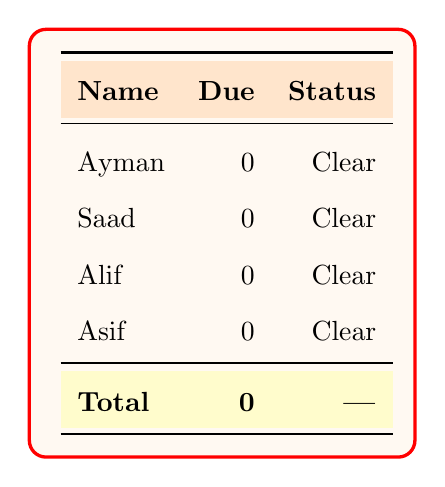
\begin{tikzpicture}
\node[draw=red, very thick, rounded corners=6pt, fill=orange!5, inner sep=8pt] {
\renewcommand{\arraystretch}{1.7}
\begin{tabular}{lrr}
\toprule
\rowcolor{orange!20}
\textbf{Name} & \textbf{Due} & \textbf{Status} \\
\midrule
Ayman  & 0  & Clear \\
Saad   & 0  & Clear \\
Alif   & 0  & Clear \\
Asif   & 0  & Clear \\
\midrule
\rowcolor{yellow!20}
\textbf{Total} & \textbf{0} & \textbf{---} \\
\bottomrule
\end{tabular}
};
\end{tikzpicture}

\end{minipage}
\hfill
\begin{minipage}{0.46\textwidth}
\normalsize
\textbf{Notes:}
\begin{itemize}[itemsep=3pt]
    \item \textbf{Have to Pay} = Meal Cost $-$ Bazar. Positive = consumed more than contributed; negative = over-contributed.
    \item \textbf{Have to Pay (Init. Cost)} = Initial Cost Rate ($63.75$) $-$ Actual Initial Cost contributed by each member.
    \item \textbf{Previous Due:} No member carries a previous due this month (all \textbf{0 BDT}).
    \item \textbf{House Rent Redistribution (15,500 BDT)} --- based on space-share fractions: Ayman $0.2823 \rightarrow 4{,}375$; Saad $0.2419 \rightarrow 3{,}750$; Alif $0.2823 \rightarrow 4{,}375$; Asif $0.1935 \rightarrow 3{,}000$.
    \item \textbf{Khala Bill (4,500 BDT), WiFi (650 BDT), Gas (460 BDT) \& Extra Pay (300 BDT)} divided equally by \textbf{4} members $\Rightarrow$ 1,125 / 162.50 / 115.00 / 75.00 each.
    \item \textbf{Rounded Final Pay:} Final payments are rounded up to round figures: Ayman $5{,}329 \rightarrow$ \textbf{5,330} ($+1$); Saad $5{,}514 \rightarrow$ \textbf{5,515} ($+1$); Alif $5{,}896 \rightarrow$ \textbf{5,900} ($+4$); Asif $4{,}672 \rightarrow$ \textbf{4,675} ($+3$) --- total rounding addition \textbf{9 BDT}; rounded total \textbf{21,420 BDT} (calculated total 21,411 BDT).
    \item \textbf{House Rent --- 15,500 BDT} \quad \textbf{Gas+WiFi --- 1,110 BDT} \quad \textbf{Khala Bill --- 4,500 BDT} \quad \textbf{Extra Pay --- 300 BDT}
\end{itemize}
\end{minipage}

\newpage

%───────────────────────────────────────────────
%  PAGE 2 — Overview & Highlights
%───────────────────────────────────────────────

\begin{center}
\LARGE\textbf{Mess Meal Management System}\\[4pt]
\Large September 2026 — Overview \& Highlights
\end{center}

\vspace{0.5cm}

\begin{table}[h]
\centering
\large
\renewcommand{\arraystretch}{1.6}
\begin{tabular}{llr}
\toprule
\rowcolor{blue!20}
\textbf{Category} & \textbf{Detail} & \textbf{Value} \\
\midrule
\rowcolor{gray!10}
Active Members              & Meal Members: 4 & 4 \\
\rowcolor{white}
Meal Rate                   & ---    & 65 BDT \\
\rowcolor{gray!10}
Bazar Rate                  & ---    & 1,582 BDT \\
\rowcolor{white}
Initial Cost Rate           & ---    & 63.75 BDT \\
\rowcolor{gray!10}
Total Meal                  & ---    & 97 \\
\rowcolor{white}
Total Meal Cost             & ---    & 6,330 BDT \\
\rowcolor{gray!10}
Total Bazar Cost            & ---    & 6,328 BDT \\
\rowcolor{white}
Total Initial Cost          & ---    & 255 BDT \\
\rowcolor{gray!10}
Khala Count                 & ---    & 27 \\
\midrule
\rowcolor{red!20}
Most Meal Consumer          & \textcolor{BrightGreen}{\textbf{Alif}} & \textcolor{red}{\textbf{36 meals}} \\
\rowcolor{white}
Most Bazar Contributor      & \textcolor{BrightGreen}{\textbf{Alif}} & \textcolor{red}{\textbf{2,234 BDT}} \\
\rowcolor{red!20}
Most Initial Cost Contributor & \textcolor{BrightGreen}{\textbf{Alif}} & \textcolor{red}{\textbf{135 BDT}} \\
\rowcolor{white}
Maximum Bazar Done By       & \textcolor{BrightGreen}{\textbf{Alif}} & \textcolor{red}{\textbf{10 trips}} \\
\rowcolor{red!20}
Maximum Initial Marketing Done By & \textcolor{BrightGreen}{\textbf{Ayman}} & \textcolor{red}{\textbf{2 trips}} \\
\rowcolor{white}
Most Money Expense By (Bazar+Initial) & \textcolor{BrightGreen}{\textbf{Alif}} & \textcolor{red}{\textbf{2,369 BDT}} \\
\bottomrule
\end{tabular}
\end{table}

\end{document}